\documentclass[12pt, a4paper]{article}
\usepackage{graphicx}
\usepackage{geometry}
\usepackage{fontspec}
\usepackage{hyperref}
\usepackage{indentfirst}
\usepackage{setspace}
\usepackage{array}
\usepackage{booktabs}
\usepackage{amsmath}
\usepackage{url}
\usepackage{subfigure}
\newcommand{\tabincell}[2]{\begin{tabular}{@{}#1@{}}#2\end{tabular}}
\geometry{a4paper, left=2cm, right=2cm, top=2.5cm, bottom=2.5cm}
\begin{document}
\begin{spacing}{1.5}
%%%%%%%%%%%%%%%%%%%%%%%%%%%%%%
%% Cover
%%%%%%%%%%%%%%%%%%%%%%%%%%%%%%
\begin{titlepage}
	\centering
	
\includegraphics[width=0.3\textwidth]{logo.pdf}\par
	\vspace{0.8cm}
	
\includegraphics[width=1.0\textwidth]{sf.png}\par
	\vspace{1.5cm}
	{\huge\bfseries What Affects the Winning Percentage of An NBA Team: An Empirical Test of Four-Factor Theory\par}
	\vspace{4cm}
	{\Large\itshape Yang, Feichi\par}
	\vfill
	{Student ID: 1601034}\par
	\vfill
	{Course Code: 454.001.201}
	\vfill
	Instructor:	\textsc{Sha, Dan}
	\vfill
% Bottom of the page
	{\large \today\par}
\end{titlepage}
\setmainfont{Times}
\setsansfont{Times} 
\linespread{2}
\begin{abstract}
The aim of this paper is to study the factors that affect the winning percentage for each team in the National Basketball Association (NBA). Four potential factors, which are, effective field goal percentage, turnover ratio, free throw attempt rate and offensive rebound percentage, are considered according to John Schuhmann’s blog. In this paper, three samples with 30 records each dating back to the Regular Season 2015-2016 are collected from the NBA official statistic website. Before a linear regression model to illustrate the relationship is developed, two dummy variables are introduced to the model to make a distinction among seasons and a Wald test is used to ensure that the Regular Season itself as an exogenous factor will not affect the winning percentage. We finally find that a team's field goal percentage, the frequency of a team goes to the free throw line and the ability to grab offensive rebounds are three positive factors toward winning percentage, meanwhile, the rate of turnovers a team averages is negatively related to the winning percentage.
\par
~\\
\noindent
\textbf{Keywords:} Linear regression, Shapiro-Wilk Test, Wald Test, White Test
\end{abstract}
\newpage
\tableofcontents
\newpage
\section{Introduction}
The National Basketball Association, NBA in short, with a history of over 70 years, is the most successful basketball association in the world and the last a few decades witnessed the fast development and style change of it. From Michael Jordan to Kobe Bryant and now to Stephen Curry and LeBron James, star players of the NBA keeps changing, but fans' love for basketball never fade.% The 2017 NBA Finals was the most watched NBA Final series on ABC averaging 20.38 million viewers. Game 7 of the 2016 NBA Finals registered the network's highest rated and most watched NBA game with an average audience of 31.02 million. It was the first basketball game to draw more than 30 million average viewers in the past 18 years.
\par
The world has already entered into an era of big data, and people have found the usefulness of the statistics and so have the participants of NBA. Every season, teams fight against each other to strive for a playoff spot and improve the winning percentage is the top priority of the team, so taking good advantage of embracing analytics is even more important. Nikolaidis(2013) built a basketball game strategy through statistical analysis of data\cite{YN}. Deshpande and Jensen(2016) estimated an NBA player’s impact on his team’s chances of winning\cite{SK}. Parker(2010) modeled basketball’s points per possession\cite{RJP}. Nevertheless, among all the works,  Schuhmann’s(2013) the four-factor theory stats that among all kinds of statistics, four advanced ones, namely effective field goal percentage, turnover ratio, free throw attempt rate and offensive rebound percentage, are the most concerned by winning teams\cite{JS}. 
\par
This paper intends to make an empirical test of the four-factor theory and our purpose is to see how does each factor affect the winning percentage of an NBA team. To do so, we collected data from three regular seasons, namely 2015-2016, 2016-2017 and 2017-2018. The game style many vary from season to season, so in order to get rid of this kind of influences we take the differences between the statistics of a team and those of its opponents into consideration. After that, we introduce two dummy variables to make a distinction among seasons and run a Wald test to ensure that the Regular Season itself as an exogenous factor will not affect the winning percentage. Finally a linear regression is established to study the relationship between the winning percentage and these four factors and thus testify the four-factor theory.
\newpage
\section{Data}
\subsection{Data Description}
All the data from Regular Season 2015-2016 to Regular Season 2017-2018 were collected from the official NBA statistic website (\url{https://stats.nba.com/}). The four factors were singled out together from all the categories to a separated table, so there were three tables (one for each season) in total. The structure of the tables is shown in Table \ref{tb1}.
\begin{table}[!h]
\centering
\setlength{\tabcolsep}{1mm}{
\begin{tabular}{ccccccccccc}
	\toprule[2pt]
	Team&WIN\%&EFG\%&\tabincell{c}{FTA RATE\%} &TOV\%&OREB\%&\tabincell{c}{OPP \\EFG\%}&\tabincell{c}{OPP\\FTA RATE\%}&\tabincell{c}{OPP\\TOV\%}&\tabincell{c}{OPP\\OREB\%}\\
	\midrule		
	Warriors&81.7&56.3&25.9&14.6&27.2&48.6& 26.1&15.4&29.1\\
	Spurs&74.4&52.4&26.3&14.1&28.2&49.2&24.9&15.1&27.0\\
	Rockets&67.1&54.5&30.4&15.0&28.1&51.9&25.0&14.9&28.3\\
	...& ... &... &... &... &... &... &... &... &... \\
	...& ... &... &... &... &... &... &... &... &... \\
	...& ... &... &... &... &... &... &... &... &... \\
	Lakers&31.7&50.1& 25.9& 15.3&28.4&54.2&27.9&14.6&28.3\\
	Suns&29.3&49.3&29.7&15.2&29.9&52.5&33.8&14.6&28.2\\
	Nets&24.4&50.7&28.9&16.2&24.1&51.3&27.5&13.0&28.4\\
	\bottomrule[2pt]
\end{tabular}}
\caption{Team Four Factors of Regular Season 2016-2017}
\label{tb1}
\end{table}
\par
Since all three tables are identical in structure, we just take the one of the Regular Season 2016-2017 as an example to illustrate the meaning of each variable. According to the four-factor theory, Effective Field Goal Percentage (EFG\%), Turnover Ratio (TOV\%), Offensive Rebound Percentage (OREB\%), and Free Throw Attempt Rate (FTA RATE\%) are essential, so they are listed in Table \ref{tb1} above. And the variables which are prefixed by the term "OPP" simply stand for the statistics of the teams' opponents. The formulas and explains of each variable are shown in Table \ref{tb2} below.

\begin{table}[!h]
\centering
\renewcommand\arraystretch{1.5}
\begin{tabular}{ccc}
	\toprule[2pt]
	Variable&Formula&Explanation\\
	\midrule		
	$WIN\%$&$\frac{WIN}{82}$&Team's winning ratio during the regular season.\\
	$EFG\%$&$\frac{FGM + 0.5 \times 3PM}{FGA}$& Team's field goal percentage.\\
	$FTA RATE\%$&$\frac{FTA}{FGA}$&It shows how often a team goes to the free throw line.\\
	$TOV\%$&$\frac{TO \times 100}{FGA + FTA \times 0.44 + AST +TOV}$& It is the rate of turnover a team averages.\\
	$OREB\%$&$\frac{OREB}{OREB + OPP OREB}$& This shows a team's ability to grab offensive rebounds.\\
	\bottomrule[2pt]
\end{tabular}
\caption{Formula And Explanation}
\label{tb2}
\end{table}
\par
In all three seasons, there were 30 teams in NBA, so 30 observations can be found in the table. Due to the length limitation, we only show 6 teams in Table \ref{tb1}.% Take the Lakers as an example, during the Regular Season 2016-2017, this team with rich history felt it hard to win a game. The Lakers only struggled to win merely 26 out of 82 games, so their winning percentage was 31.7\%. Their effective field goal percentage was 50.1\%, while the effective field goal percentage of their opponents was 4.1\% higher, meaning that the Lakers team was shooting worse than their opponents. The opponents of the Lakers were averaging 27.9\% free throw attempt rate, 2.0\% better than the Lakers. Also, the Lakers team was 0.7\% worse than its opponents in the term of turnover control. But this teams was better at grabbing an offensive rebound.
\par
\subsection{Data Transformation}
Each independent variable mentioned above can be affected by many other exogenous factors. For instance, if both the team and its opponent are not defensively aggressive, the effective field goal percentage of both team can be fairly high and the free throw attempt rates can be rather low. But after all, the team which surpassed its opponent has a larger chance to win the game. Therefore, what really matters is the relative number, rather than the absolute value. In order to eliminate the influence of the exogenous factors and get the relative value, we calculate the differences between the statistics of a team and those of its opponents. Equation (\ref{eq1}) to Equation (\ref{eq4}) demonstrate this process.
\begin{small}
\begin{align}
	\centering
	dEFG &= EFG\% - OPP\ EFG\% \label{eq1}\\
	dFTA &= FTA\ RATE\% - OPP\ FTA\ RATE\% \label{eq2}\\
	dTOV &= TOV\% - OPP\ TOV\% \label{eq3}\\
	dOREB &= OREB\% - OPP\ OREB\% \label{eq4}
\end{align}
\end{small}
\par
After the data transformation, eight variables are reduced into four and the data structure is shown below in Table \ref{tb3}. Again, we only single out four teams from Regular Season 2016-17 for demonstration.
\par
\begin{table}[!ht]
\centering
\setlength{\tabcolsep}{2mm}{
\begin{tabular}{cccccccccc}
	\toprule[2pt]
	Team&WIN&dEFG&dFTA&dTOV&dOREB\\
	\midrule		
	Warriors&81.7&56.3&25.9&14.6&27.2\\
	Spurs&74.4&52.4&26.3&14.1&28.2\\
	...& ... &... &... &... &... \\
	Suns&29.3&49.3&29.7&15.2&29.9\\
	Nets&24.4&50.7&28.9&16.2&24.1&\\
	\bottomrule[2pt]
\end{tabular}}
\caption{The Difference of Four Factors from Regular Season 2016-2017}
\label{tb3}
\end{table}
% \newpage
\section{Model}
The goal of our project is to figure out how each factor influences the winning percentage of a basketball team in NBA. In our research, a Wald test is conducted so as to ensure data of three seasons can be combined together  and also a linear regression model is developed with Python library DaPy and the model assessment indices are  $R^2$ and $RMSE$.
\subsection{Linear Regression}
We assume that variable $Y (winning\ percentage)$  can be explained by variables $X_1\,(dEFG)$, \\$X_2\,(dFTA)$, $X_3\,(dTOV)$ and $X_4\,(dOREB)$, and the relationship between them can be defined as linear relation. Moreover, we assume that unpredictable variable $\epsilon$ is under normal distribution with mean 0 and variance $\sigma^2$. As mentioned earlier, the game style may change from season to season therefore the model is not accurate when we establish it with combinational data (observations from three seasons) if the influence of exogenous factors is significant. In order to recognize the impact of the variables other than the four factors, we introduce the dummy variables $D_i$ of seasons. The entire model is developed as Equation (\ref{eq77}),
\begin{equation}
\label{eq77}
\begin{split}
WIN=&\beta{X^{'}}+\epsilon=\beta(X+D+X\cdot{D})+\epsilon\\
=& \beta_0+\beta_1dEFG + \beta_2dFTA+\beta_3dTOV+\beta_4dOREB \\
&+ \beta_5D_{1516}+\beta_6D_{1617}\\
&+\beta_7D_{1516}dEFG+\beta_8D_{1516}dFTA+\beta_9D_{1516}dTOV+\beta_{10}D_{1516}dOREB\\
&+\beta_{11}D_{1617}dEFG+\beta_{12}D_{1617}dFTA+\beta_{13}D_{1617}dTOV+\beta_{14}D_{1617}dOREB + \epsilon \\
\end{split}
\end{equation}
where, 
$\beta_0$ represents the constant item in the method;
$\beta_i,\ i=1, 2, \cdots, 14$ represents the coefficients of each variable;
$D_{1516}, D_{1617}$ represents the dummy variable of season 2015-2016 and 2016-2017.

After the model is developed, it is necessary to testify that the model satisfies all the assumptions. The test involves four steps. Firstly, the normality of the residual should be tested. Secondly, we calculate the Spearman correlation between the independent variables and residual error in attempt to check whether the residual are characterized with heteroscedasticity. Thirdly, we compute the D-W stats to check the autocorrelation. Finally, the variance inflation factor (VIF) is applied to diagnose the multiple-collinearity.
\subsection{Wald Test}
Wald test is used to detect whether season-related variables in the model have significant effects. We settle down the null hypothesis for this test is: all of the parameters which related to the seasons equal to zero. The meaning of null hypothesis can be presented by Equation (\ref{eq100}).
\begin{equation}
	H_0: \beta_5=\beta_6=\cdots=\beta_{14}=0
	\label{eq100}
\end{equation}
\subsection{The Shapiro-Wilk Test of Normal Distribution}
It needs special attention that after one linear regression model is estimated, its residual should be tested to check whether it is normally distributed.

The Shapiro-Wilk test (S-W test) is one of the most frequently used methods to test the normality of random variables. The null hypothesis states that the sample $x_1$, ..., $x_n$ comes from a normally distributed population \cite{SW}. The statistic of this test is written in Equation (\ref{eq9}):
\begin{equation}
	W=\frac{(\sum_{i=1}^na_ix_{(i)})^2}{\sum_{i=1}^n(x_i-\bar{x})^2}	
	\label{eq9}
\end{equation}
and the coefficients $a_i$ are given by:
\begin{equation}
	(a_1, ...,a_n)=\frac{m^{T}V^{-1}}{(m^TV^{-1}V^{-1}m)^{\frac{1}{2}}}	
	\label{eq10}
\end{equation}
where, $x_{(i)}$ is the number i order statistic;
$\bar{x}$ is the sample mean;
$m = (m_1, \cdots, m_n)^T$ is a vector made of the expected values of the order statistics of independent and identically distributed random variables sampled from the standard normal distribution;
$V$ is the covariance matrix of those order statistics.
\subsection{Model Assessment}
\subsubsection{Coefficient of Determination $R^2$}
The coefficient of determination is the proportion of the variance in the dependent variable that is predictable from the independent variables and in most case, the higher the proportion is, the better the regression is. The coefficient of determination ($R^2$) is defined in Equation (\ref{eq11}),
\begin{equation}
	R^2 = \frac{\sum_{i=0}^N(\hat{y_i}-\bar{y})^2}{\sum_{i=0}^N(y_i-\bar{y})^2}
	\label{eq11}
\end{equation}
where, $\hat{y_i}$ is the predict value of the i-th observation and $\bar{y}$ is the mean of the variable $y$.
\subsubsection{Adjusted $R^2$}
However, when a model has more than one variable, the $R^2$ increases as the number of variables increases. This misleads people to choose models with as many independent variables as possible. In contrast to models with fewer independent variables, those with more variables are often unstable. In our case, simply using $R^2$ may misleads us to choose the model with four variables, even if a model with two variables is already good enough. To avoid problems like this, we adopt adjusted $R^2$ as the measure of goodness of fit. The mathematical definition of adjusted $R^2$ is given in Equation (\ref{eq12}),
\begin{equation}
	Adj-R^2 = 1 - \frac{n-1}{n-p-1}(1-R^2)
	\label{eq12}
\end{equation}
where $n$ equals to the number of the observations and $p$ equals to the number of variables.
\subsubsection{Root-Mean-Square Error}
Another commonly used statistic used to assess the performance of a model is root-mean-square error (RMSE). It directly shows the accuracy of its prediction. Its mathematical definition is written in Equation (\ref{eq13}).
\begin{equation}
	RMSE = \sqrt{\sum_{i=1}^n{(\hat{y_i}-\bar{y})^2}}
	\label{eq13}
\end{equation}
% \newpage
\section{Results}
\subsection{Model With Exogenous Factors}
Least Square Method is applied to estimate the parameters in Equation \ref{eq77}. And the result is shown below in Equation \ref{eq88}.
\begin{equation}
\label{eq88}
\begin{split}
WIN=& 49.96+5.23dEFG + 0.60dFTA-3.57dTOV+1.61dOREB \\
&+ 0.01D_{1516}-0.06D_{1617}\\
&-0.56D_{1516}dEFG-0.31wD_{1516}dFTA-0.65D_{1516}dTOV+0.38D_{1516}dOREB\\
&-0.54D_{1617}dEFG-0.21D_{1617}dFTA-0.05D_{1617}dTOV+0.01D_{1617}dOREB + \epsilon \\
\end{split}
\end{equation}

\subsubsection{Test of the Assumptions}
\begin{itemize}
\item[(1)] \textbf{Normality of the residual.} The S-W statistic is 0.990 and its p-value is 0.711 which is more than 0.05. So we accept the null hypothesis that the residual is normally distributed\cite{NORMAL}.
\item[(2)] \textbf{Autocorrelation of the residual.} The D-W statistic is the most common way to judge whether the residual series are autocorrelated. The statistic of D-W test is 1.956, which means that the residual series are not autocorrelated.
\item[(3)] \textbf{Heteroscedasticity of the residual}. B-P test is introduced here to test the heteroscedasticity\cite{9}. The p-value is 0.4572 which is greater than the 0.05 level. So we accept the null hypothesis that there is no heteroscedasticity of the residual.
\item[(4)] \textbf{Test of Multi-collinearity}. When there are multiple collinearities among independent variables, the estimated values of regression parameters obtained by ordinary least squares method will not be the best linear unbiased estimator (BLUE) of the coefficients.  Variance inflation factor (VIF) is always used as a diagnostic method. Table \ref{tb99} shows that the VIFs of each coefficients are all smaller than 10\cite{9}. So we believe that there is no multi-collinearity between independent variables.
\begin{table}[!ht]
\centering
\setlength{\tabcolsep}{8mm}{
\begin{tabular}{cccccccc}
	\toprule[2pt]
	Variable&Tolerance&VIF\\	
	\midrule
	$dEFG$&.261&3.829\\
	$dFTA$&.346&2.886\\
	$dTOV$&.286&3.491\\
	$dOREB$&.198&5.043\\
	$dD_{1516}$&.750&1.333\\
	$dD_{1617}$&.720&1.334\\
	$dEFG_{1516}$&.381&2.624\\
	$dFTA_{1516}$&.544&1.837\\
	$dTOV_{1516}$&.401&2.497\\
	$dOREB_{1516}$&.300&3.332\\
	$dEFG_{1617}$&.436&2.291\\
	$dFTA_{1617}$&.466&2.145\\
	$dTOV_{1617}$&.446&2.240\\
	$dOREB_{1617}$&.336&2.978\\
	\bottomrule[2pt]
\end{tabular}}
\caption{Collinearity Statistics}
\label{tb99}
\end{table}
\end{itemize}
\newpage
\subsubsection{The Result of Wald Test}
Since our aim is to verify the influence of any exogenous factors, the null hypothesis is $\beta_5=\beta_6=\cdots=\beta_{14}=0$. The result of the Wald test shows that the F-statistic is 0.449141 and the p-value is  0.9168, so we accept the null hypothesis.

This result means that the influence of the differences among seasons is not significant. So it is reasonable to consider the three samples as one with 90 observations.

Therefore, the model can be written as:
\begin{equation}
	WIN = \beta_0+\beta_1dEFG + \beta_2dFTA+\beta_3dTOV+\beta_4dOREB + \epsilon
\end{equation}

\subsection{The Final Model}
Least Square Method is applied to estimate the parameters and the result is shown below in Equation (\ref{eq129}). The $R^2$ of this model is 91.80\% and the $Adj-R^2$ is 91.41\%.

\begin{equation}
	WIN=49.9473 + 4.85dEFG+0.44dFTA-3.76dTOV+1.74dOREB
	\label{eq129}
\end{equation}
\subsubsection{Test of the Assumptions}
\begin{itemize}
\item[(1)] \textbf{Normality of the residual.} We use the Shapiro-Wilk test to check the normality the residual and the result is shown in Table \ref{tb9} \cite{A}. The table illustrates that all four p-values excess the threshold of .05, meaning that we accept the null hypothesis that the variables are normally distributed.
\begin{table}[!ht]
\centering
\setlength{\tabcolsep}{10mm}{
\begin{tabular}{cccccccccc}
	\toprule[2pt]
	\,&Statistic&df&p-value\\
	\midrule		
	residual&.993&90&.939\\
	\bottomrule[2pt]
\end{tabular}}
\caption{The Result of the Shapiro-Wilk Test}
\label{tb9}
\end{table}\item[(2)] \textbf{Autocorrelation of the residual.} The statistic of D-W test is 2.0469, which means that the residual series are not autocorrelated.
\item[(3)] \textbf{Heteroscedasticity of the residual}. There are two ways to check whether heteroscedasticity exists. 

\begin{itemize}
\item[1.] One of the most intuitive and convenient analysis ways is to draw the residual graph. We plot the residual graph and the scatter plots of residual with independent variables (See Figure \ref{fig1}).

\begin{figure}[h]
	\centering  
	\subfigure{
	\begin{minipage}[ht]{2.6in}
	\centering
	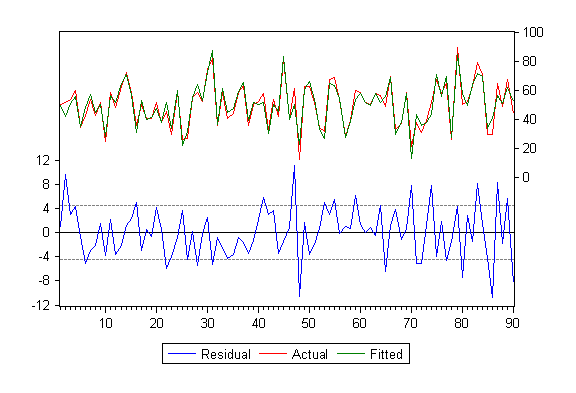
\includegraphics[width=1\linewidth]{figures/figure2.png}
	%\caption{fig1}
	\end{minipage}%
	}%
	\subfigure{
	\begin{minipage}[ht]{2.6in}
	\centering
	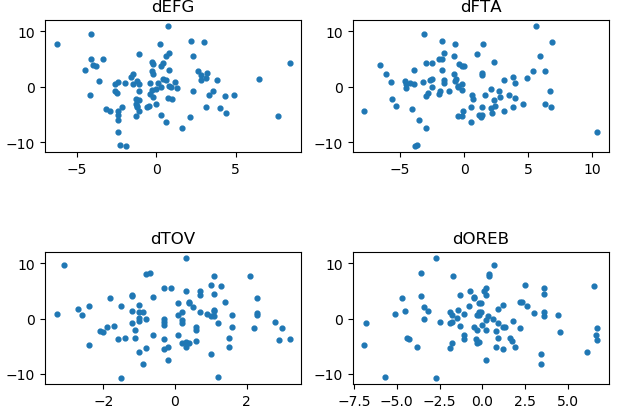
\includegraphics[width=1\linewidth]{figures/figure1.png}
	%\caption{fig2}
	\end{minipage}%
	}%
	\caption{The Residual Graph and Scatter Plots.}
	\label{fig1}
\end{figure}

We can clearly see that the residual is normally distributed and the dots are randomly and irregularly scattered in the scatter plots, and they do not show any trend. So we think that the residual has no heteroscedasticity.

\item[2.] In addition, calculating the spearman correlation between residual error and independent variables is the second way to check heteroscedasticity. The correlations between independent variables and residual error are not significant. By now, no heteroscedasticity has been detected. The detail of this test is shown in Table \ref{tb7}.

\begin{table}[!ht]
\centering
\setlength{\tabcolsep}{6mm}{
\begin{tabular}{cccccccc}
	\toprule[2pt]
	Variable&Spearman&t&p-value\\	
	\midrule
	dEFG&-0.0888&-0.8363&0.4052\\
	dFTA&0.1161&1.0965&0.2758\\
	dTOV&0.0021&0.0197&0.9844\\
	dOREB&0.0559&0.5252&0.6008\\
	\bottomrule[2pt]
\end{tabular}}
\caption{Residual Correlation}
\label{tb7}
\end{table}
\end{itemize}
\item[(4)] \textbf{Test of Multi-collinearity}. Table \ref{tb50} shows that the VIFs of each coefficients are all smaller than 10. So we believe that there is no multi-collinearity between independent variables.
\begin{table}[!ht]
\centering
\setlength{\tabcolsep}{8mm}{
\begin{tabular}{cccccccc}
	\toprule[2pt]
	Variable&Tolerance&VIF\\	
	\midrule
	(Constant)&\,&\,\\
	dEFG&.954&1.049\\
	dFTA&.955&1.047\\
	dTOV&.944&1.060\\
	dOREB&.903&1.107\\
	\bottomrule[2pt]
\end{tabular}}
\caption{Collinearity Statistics}
\label{tb50}
\end{table}
\end{itemize}
% \newpage
\subsubsection{Interpretation of the Coefficients}
The coefficients in the model are estimated, then the t-test is applied to test the significant of parameters in the model. The coefficients' failure to pass the t-test means that their influence is not significant in the model. To simplify the model, the useless independent variables were deleted. Finally, the model is developed as Equation (\ref{eq14}).
\begin{equation}
	WIN=49.9473 + 4.85dEFG+0.44dFTA-3.76dTOV+1.74dOREB
	\label{eq14}
\end{equation}
\par
In summary, a team's field goal percentage, the frequency of a team goes to the free throw line, the ability to grab offensive rebounds are three positive factors toward winning percentage. However, the rate of turnover a team averages is negative to the winning percentage. This equation can also interpret the following findings:

\begin{itemize}
\item[(1)] The constant (49.9473) in the equation means that if the team performs as well as its opponents in all aspects (EFG, FTA, TOV and OREB), the winning percentage of this team will be 49.9473\% (about 50\%) in this regular season. 
\item[(2)] If team's field goal can be 1 percentage better than its opponents, the overall winning percentage of this team will increase 4.85\% in regular season.
\item[(3)] If the frequency of a team goes to the free throw line is 1\% more than its opponents, the overall winning percentage of this team will increase 0.44\% in regular season.
\item[(4)] If the ability to grab offensive rebounds is 1\% greater than its opponents, the overall winning percentage of this team will increase 1.74\% in regular season.
\item[(5)] If the turnover rate a team average is 1\% higher than its opponents, the overall winning percentage of this team will decrease 3.76\% in regular season.
\end{itemize}
% \newpage
\section{Conclusion and Discussion}
This paper intends to have an empirical test of four-factor theory, we download data from the official NBA statistic website and get three four-factor tables, each table containing 30 observations, for Regular Season 2015-2016, Regular Season 2016-2017 and Regular Season 2017-2018. So as to avoid the impact of other exogenous factors, we reduce eight variables into four by taking the differences between the statistics of a team and those of its opponents. Then we utilize Wald Test make sure that it is reasonable combine three samples into one with 90 observations. Finally, we use linear regression to establish a model to study what and how factors affect the winning percentage of an NBA team.

However, there are some obvious short-comes in our work. The first one is that our model cannot explain and predict the outcome of a single game. For example, the model cannot tell the fans whether the Lakers or the Warriors will win the Western Conference final Game 7. The second one is that due to the abstractness of the variables, our model cannot directly lead to modifications of tactics.

In the future work, we would like to combine the data from more than three seasons so that we are able to gain an even larger sample size. The reality may not always be linear, developing a non-linear model is worth considering. Also a model which can be used to predict the outcome of a single game is more practical and in this case Neural Network Models may be helpful.
\newpage
\begin{thebibliography}{}
	\bibitem[1]{YN}	Yiannis Nikolaidis. (2013). Building a basketball game strategy through statistical analysis of data. Springer Science+Business Media New York. Ann Oper Res (2015) 227: 137-159. DOI 10.1007/s10479-013-1309-4.\\
	\bibitem[2]{SK}	Sameer K. D. \& Shane T. J. (2016). Estimating an NBA player's impact on his team's chances of winning.\\
	\bibitem[3]{RJP} Ryan J. P. (2010). Modeling Basketball's Points per Possession With Application to Predicting the Outcome of College Basketball Games. Bachelor, College of Charleston.\\
	\bibitem[4]{JS}	John Schuhmann. (2013). The New NBA.com/stats: Advanced Stats All Start with Pace and Efficiency. sci: http://hangtime.blogs.nba.com/2013/02/15/the-new-nba-comstats-advanced-stats-all-start-with-pace-and-efficiency/.\\
	\bibitem[5]{LR} HE X. \& LIU W. (2015). \*Applied Regression Analysis\*. Beijing: Renmin Publisher.\\
	\bibitem[6]{NORMAL} Kankainen, A., Taskinen, S., \& Oja, H.. On Mardia's Tests of Multinormality. (1991). *Mathematics Subject CLassification*. N.D.\\
	\bibitem[7]{SW} Shapiro, S. S., Wilk, M. B. (1965). *An analysis of variance test for normality (complete samples)*. Biometrika. 52 (3-4): 591:611. \\
	\bibitem[8]{A} JMP. (2004). *How do I interpret the Shapiro-Wilk test for normality in JMP*. N.D.\\
	\bibitem[9]{9} HE X; LIU W. Applied Statistic. Applied Regression Analysis. China People University Publisher: Beijing, China, 2015; pp. 91-132.

\end{thebibliography}

\end{spacing}
\end{document}